\documentclass[aspectratio=1610,svgnames]{beamer}

\usepackage{lmodern}
\usepackage[T1]{fontenc}
\usepackage[ngerman]{babel}
\usepackage{selinput}
\SelectInputMappings{%
   adieresis={ä},
   germandbls={ß}
   }

\usetheme{PaloAlto}  %% Themenwahl

\setbeamercovered{transparent}
%\setbeamertemplate{footline}[frame number]
\usecolortheme{spruce}		% grün
\usecolortheme[named=MSUgreen]{structure}
\newcommand{\hshblogo}{
\includegraphics[width=1.3cm]{space-logo}}
\newcommand{\divider}[1]{\begin{frame} %
\begin{alertblock}{} %
\centering\usebeamerfont{section title}#1 %
\end{alertblock} %
\end{frame}}
 
\newcommand{\code}[1]{\texttt{#1}}

\title{3D Objekte mit OpenSCAD}
\author{Thomas Helmke}
\date{09.02.2016}
\logo{
\includegraphics[width=1.1cm]{space-logo}}
 
\begin{document}
\maketitle
\frame{\tableofcontents}

\section{Einleitung}
\divider{\insertsection}
\begin{frame}%[<+->] %%Eine Folie
	\frametitle{Worum geht es?} %%Folientitel
	\begin{itemize}
		\item 3D Objekte entwerfen
        \item 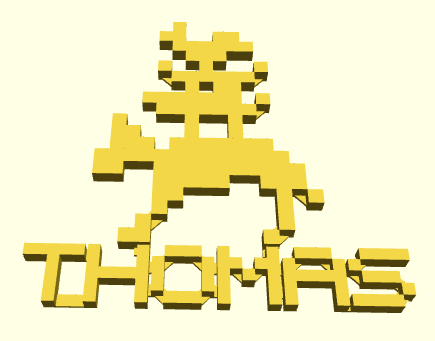
\includegraphics[width=0.3\textwidth]{nametagthomas}
		\item zum Beispiel für 3D Druck
	\end{itemize}
\end{frame}
\begin{frame}[<+->] %%Eine Folie
	\frametitle{openSCAD} %%Folientitel
	\begin{itemize}
		\item eine 3D CAD Software
        \item nicht interaktiv, sondern skriptbasiert
		\item freie Software, für alle Platformen erhältlich\footnote{\url{www.openscad.org}}
		\item fast vollständige JavaScript Version läuft direkt im Browser\footnote{\url{www.openscad.net}}
	\end{itemize}
\end{frame}

\section{Grundlagen}
\divider{\insertsection}
\subsection{Basiskörper}
\divider{\insertsubsection}
\begin{frame}[<+->]
    \frametitle{Basiskörper}
    \begin{itemize}
        \item Würfel -- \code{cube([xLänge, yLänge, zLänge]);}
        \item Zylinder -- \code{cylinder(h = Höhe, r1 = RadiusUnten, r2 = RadiusOben);}
        \item Kugel -- \code{sphere(r = Radius);}
    \end{itemize}
\end{frame} 
\begin{frame}[<+->]
    \frametitle{optionale Parameter}
    \begin{itemize}
        \item \code{center} -- zentriert den Körper im Koordinatenursprung
        \item \code{\$fn} -- Anzahl der Flächen für runde Körper
        \item \code{d} -- Durchmesser statt Radius
    \end{itemize}
\end{frame} 
\subsection{Basisoperationen}
\divider{\insertsubsection}
\begin{frame}[<+->]
    \frametitle{Basisoperationen}
    \begin{itemize}
        \item Verschieben -- \code{translate([x, y, z])}
        \item Rotieren -- \code{rotate([xGrad, yGrad, zGrad])}
        \item Skalieren -- \code{scale([xFaktor, yFaktor, zFaktor])}
        \item Spiegeln -- \code{mirror([x,y,z])}
    \end{itemize}
\end{frame} 
\begin{frame}[<+->]
    \frametitle{Beispiel}
    \code{translate([2,3,4])\newline%
        \hspace*{1em}rotate([45,0,0])\newline%
        \hspace*{2em}scale([0.5,1,2])\newline%
        \hspace*{3em}cube([1,1,1]);}
\end{frame} 

\section{Fortgeschrittene Techniken}
\divider{\insertsection}
\subsection{Variablen}
\divider{\insertsubsection}
\begin{frame}[<+->]
    \frametitle{Variablen I}
    \begin{itemize}
        \item Werte können in Variaben gespeichert werden
        \item Variablen können mathematisch verrechnet werden
    \end{itemize}
    \uncover<+->{%
    \code{xsize = 3.5;\newline%
        ysize = xsize;\newline%
        zsize = 0.5*xsize;}}
\end{frame}
\begin{frame}[<+->]
    \frametitle{Variablen II}
    \begin{itemize}
        \item Variablen können an Funktionen übergeben werden
    \end{itemize}
    \uncover<+->{%
    \code{translate(v=[xpos*(gap+xsize)+0.5*xsize,ypos*(gap+ysize)+0.5*ysize,0.5*zsize])\newline%
        \hspace*{1em}cylinder(h=1.1*zsize, r=0.4*xsize, \$fn=20, center=true);}}
\end{frame}
\begin{frame}[<+->]
    \frametitle{Module I}
    \begin{itemize}
        \item beliebige Funktionen zu Modulen zusammenfassen
        \item Wiederverwendbarkeit von Code
        \item Module können in externe Dateien ausgelagert werden
    \end{itemize}
\end{frame}
\begin{frame}[<+->]
    \frametitle{Module II}
    \begin{itemize}
        \item -
        \item -
        \item -
    \end{itemize}
\end{frame}

\section{Scripting}
\divider{\insertsection}
\begin{frame}[<+->]
    \frametitle{Python}
    \begin{itemize}
        \item .
        \item .
        \item .
        \item .
    \end{itemize}
\end{frame}

\section{Weitere Infos}
\divider{\insertsection}
\begin{frame}
    \frametitle{Weitere Infos}
    \begin{itemize}
        \item \url{https://github.com/Syralist/hshb-pres-openscad}
        \item \url{http://www.openscad.org}
        \item \url{http://www.openscad.net}
        % \item \url{https://gist.github.com/jh0ker/8a63a66d368d7b48c89d}
    \end{itemize}
\end{frame}
\end{document}
